%
% File acl2012.tex
%
% Contact: Maggie Li (cswjli@comp.polyu.edu.hk), Michael White (mwhite@ling.osu.edu)
%%
%% Based on the style files for ACL2008 by Joakim Nivre and Noah Smith
%% and that of ACL2010 by Jing-Shin Chang and Philipp Koehn
\documentclass[11pt]{article}
\usepackage{acl2012}
\usepackage{times}
\usepackage{latexsym}
\usepackage{amsmath}
\usepackage{multirow}
\usepackage{url}
\usepackage{graphicx}
\DeclareMathOperator*{\argmax}{arg\,max}
\setlength\titlebox{6.5cm}    % Expanding the titlebox

\title{Detecting English Writing Styles For Non Native Speakers}

\author{Rami Al-Rfou', Yanging Chen, Yejin Choi \\
  Department of Computer Science \\
  Stony Brook University \\
  NY 11794, USA \\
  {\tt \{ralrfou, cyanqing, ychoi\}@cs.stonybrook.edu}}

\date{1/6/2012}

\begin{document}
\maketitle
\begin{abstract}
This paper presents the first attempt (up to our knowledge) to classify English writing styles of non native speakers on this scale. Classifying day to day written language of writers with different backgrounds covering various areas of topics is a real challenge.The paper proposes simple machine learning algorithms and simple to generate features to solve the challenge. Relying on the scale of the data available from large sources of knowledge like Wikipedia. We believe such sources of data are crucial to generate robust solutions for the web with high accuracy and easy to deploy in practice. The paper achieves 74\% accuracy classifying native versus non native speakers writing styles.

Moreover, the paper shows some interesting observations on the similarity between different languages measured by the similarity of their users English writing styles. This technique could be used to support some well known linguistic theories about the languages families and their origins.
\end{abstract}



\section{Introduction}
The internet nowadays is more diverse than any time before. The introduction of social networks changed the distribution of users; the majority of users are not any more native English speakers. This puts more challenges on the services providers to accommodate the English content to the new users. This paper tackles the challenge of identifying the native language of the user from their writing styles. We believe this task is crucial as a first step in the development of many useful applications.

Wikipedia is well known source of knowledge. Recently, it is used extensively to help solving different information retrieval tasks especially the ones that involves semantic aspects. The use of Wikipedia can be expanded to help the common NLP tools to perform better with the help of the diversity of topics and authors of Wikipedia pages. The large size of encyclopedia can help in the data sparsity problem. Moreover, the sustained growth of Wikipeida content of can bring performance gains with no much additional complexity costs.

The detection of the writer's native language can be helpful in application that targets new learners of English as a second language. Moreover, it could be adapted to transcribed text to help better voice recognition application when dealing with the non native speakers accents.

\section{Related Work}
The first work related with native language identification is that of \cite{koppel2005automatically}, in which they tried profiling anonymous authors with their native languages. Totally five different groups of English authors (whose native languages are Russian, Bulgarian, French, and Spanish) were picked from the first version of {\em International Corpus of Learner English} (ICLE) in their experiments. By applying a combined feature sets, including function words, character n-grams, part-of-speech bi-grams and spelling mistakes, they gained an accuracy of 65\% if considered style features only. These results suggested that syntactic features are valuable when trying to categorize authors by their native languages. Also in \cite {koppel2005determining}, they considered not only letter n-grams and function words but errors and idiosyncrasies, including orthography errors, syntax errors, neologisms and part-of-speech bigrams errors. Finally the accuracy on classifying authors from five different countries can reach above 80\%. \cite {argamon2009automatically} concluded some more important features in the task of profiling authors of an anonymous text.

Similar work was done by \cite {tsur2007using}. They focused on the relationships between choice of words in second language writing and the frequency of native language syllables, also known as the phonology of native languages. \cite {estival2007author} studied a wide range of lexical and document structure features in their native languages classification task. And \cite {zheng2003authorship}, though they did not directly conduct related experiments on nationality detection, they provide some features of style marks that could be used in the task of judging one's native languages. Besides, \cite {gamon2004linguistic} analyzed the power of some general features under different frequency cutoffs. But none of these measured the usefulness of syntactic features under a general condition for the task of native language detection.

\cite {wong2009contrastive} replicated the work of \cite {koppel2005automatically} and dug more in the field of syntactic structures. They experimented on three selected syntactic errors, which are commonly observed in non-native English Users, including subject-verb disagreement, mismatch of noun-number pairs and wrong usage of determiners and the best overall accuracy was 73.71\% on the second version of ICLE across seven languages. \cite {wong2010parser} first considered applying parser features in the task--though these features are hard to extract compared with other syntactic features. What's more, \cite {wong-dras:2011:EMNLP} continued their works in native language detection and focused more on the influence of syntactic structures, specifically parsing trees. They tried to exploiting the parsing structures by applying Standford parsers and C\&J parsers with different parameters to certain corpus, and capture the number of usages of some distinguishable rules. Their results and observations suggested that the syntactic structures would be supportive in detecting native languages and improving the performance of existing classifiers.

Different from previous works mentioned above, our task runs on a totally different platform--wikipedia. Our goal is to find out the influence of one's native languages on the style of his/her writings under the circumstance of talking and discussion. With the help of huge amount of available data, we can try exploring the statistics features of a certain languages using similar features in \cite {koppel2005automatically} and \cite {wong-dras:2011:EMNLP}, as well as the distribution of part-of-speech(PoS) n-grams and word n-grams.      

\section{Wikipedia}
Wikipedia is the de facto source of knowledge for internet users. Wikipedia is the 5\textsuperscript{th} most popular website according to Google ranking. For researchers Wikipedia is a giant linguistic and social jar of experiments. The richness of the website content that is written by users from different backgrounds represents a robust sample of the current languages usage by native and non native speakers.

With more than 90 thousand active users and 4.4 million article, the content of Wikipedia spans large number of topics. The diversity of authors beside the records of versions that are stored in a database of revisions presents a realistic source of text. Such resource presents a higher quality of data that is not achievable by the other commonly used sources of text as news, blogs and scientific articles.

Such successful website has a complex database structure to serve its users. Therefore, extracting data is a complex process. Our goal is to identify the languages skills of the users and collect their contributions. To achieve the first task Wikipedia has an information box called \emph{Babel} that users can add voluntarily to their profile pages to state their skills in different languages. Figure \ref{babel} shows a user who identified her native language and her skills in 3 other non native languages on a scale of 1-5. This info box is indexed in the database as categories.

\begin{figure}[htp]
\centering
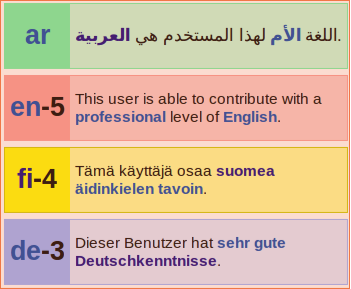
\includegraphics[scale=0.60]{babel}
\caption{Wikipedia languages skills info box (Babel)}
\label{babel}
\end{figure}

The task of collecting the contributions of a specific user is more complex procedure. The diffs between Wikipedia pages revisions has to be generated and linked back to the user table. However, the resources we have to process such huge amount of data did not allow us to do that\footnote{Recent efforts were made to generate the diffs \url{http://dumps.wikimedia.org/other/diffdb/}}. Instead we noticed that Wikipedia pages have accompanying discussion pages where users discuss different aspects of the articles. In those pages the tradition is to sign the user comments with a signature that link back to the user. Figure \ref{obama} shows an example of those comments. The style of writing of those talk pages are less formal and technical than the main pages of Wikipedia and has more conversational stylistic features.

\begin{figure*}[Htp]
\centering
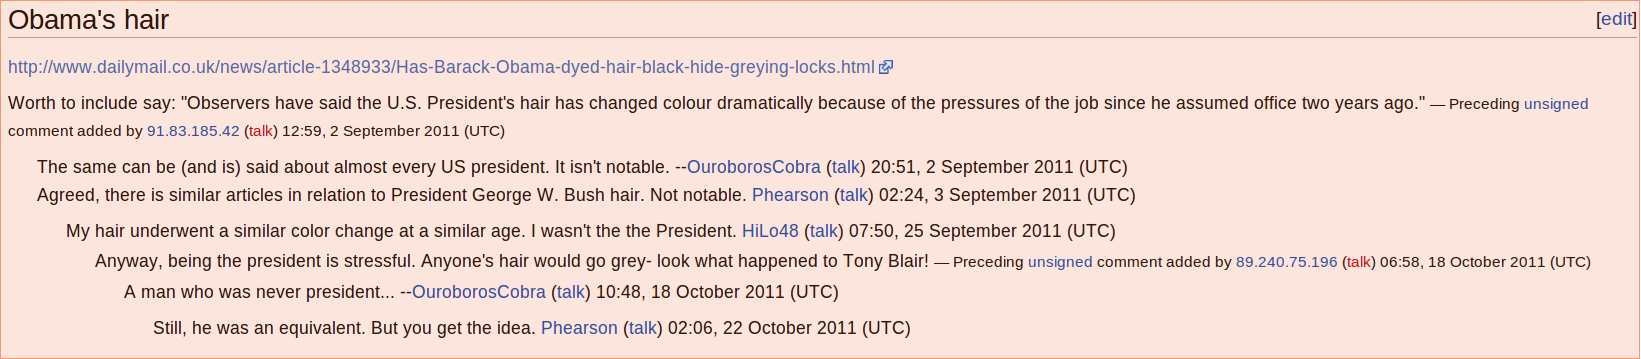
\includegraphics[scale=0.285]{obama.png}
\caption{Example of a conversation in the discussion pages}
\label{obama}
\end{figure*}

The recommended signatures patters are limited, however, in practice the users use various patterns that makes the detection rules ambiguous. The detection algorithm implemented relies on complex regular expressions and applies best effort strategy.

\section{Experiments}
We found that around 60 thousands users specified their language skills. Figure \ref{native_dist} shows that the percentage of users who claimed that their native language is English is around 47\% of English Wikipedia users base.

\begin{figure}[htp]
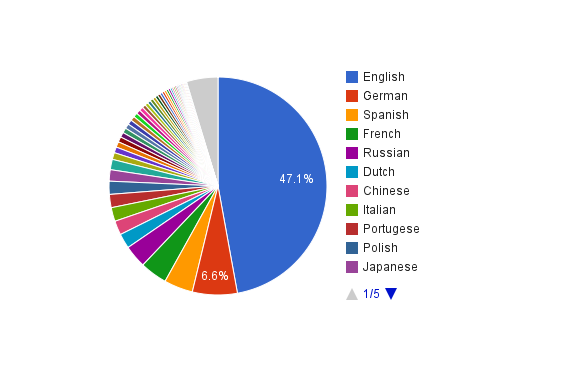
\includegraphics[scale=0.56]{chart_4.png}
\caption{Users distribution over native languages in English Wikipedia}
\label{native_dist}
\end{figure}

We parsed the talk pages with the \verb+namespace=1+, they represents more than 80\% of the talk pages, which produced around 12 million comments. Only 2.4 million comment we could identify them to belong to users with known language skills. As not all the users contributes to the talk pages, the number of users who makes at least one comment in the extracted comments is around 30 thousand user.

Since we have large number of comments and users, we can apply more filtering to increase the quality of data gathered. Therefore, we applied the following filtering mechanisms:
\begin{itemize}
\item Users are grouped according to their native languages. Users of the most frequent 20 native languages are selected.
\item Only US English native speakers are selected. This made to avoid the variations of standard English among different dialects and countries. Moreover, this step helps to filter the non native speakers who are proficient in English so they choose the general Native English category in their skills.
\item Users who specified more than one native language are excluded. This step helps to avoid unrealistic scenarios where users claim to be native in more than one language.
\end{itemize}

The new data set after the filtering is composed of 9857 user and 589228 comments.

\subsection{Setup}
The following experiments are conducted under the following conditions:
\begin{itemize}
\item The accepted comments have to have at least 20 tokens.
\item Proper nouns are replaced by their tags to avoid bias toward topics.
\item Non ASCII characters are replaced by a special character to avoid bias toward non English characters usage in the comments.
\item The classifier has balanced number of comments for each of its classes. Therefore, the two baseline classifiers; the most common label and the random classifier will have an accuracy of \verb+1/number of classes+.
\item The data set is split to 70\% training set, 10\% development set and 20\% testing set.
\end{itemize}

\subsection{Features}
The comments of the training set is grouped by class and the following frequency distributions are calculated for each class:
\begin{itemize}
\item 1-4 grams over the comments words.
\item 1-4 grams over the comments characters.
\item 1-4 grams over the part of speech tags.
\end{itemize}

For each comment ($C$) similarity measurements ($Sim$) are calculated against each n-gram frequency distribution ($f(n)$) according to the following equations:

\[
  count(x, f, n) = \left\{ 
  \begin{array}{l l}
    FreqDistCount(x, f, n), & \\\quad \text{if $x$ is in $f(n)$}\\
    1,&\\\quad \text{if $x$ is not seen before}\\
  \end{array} \right.
\]
\[
  Sim(C,f,n) = \sum_{x \in ngrams(C,n)} \log_2 (count(x,f,n))
\]

Therefore, if the problem has six classes, this will generate $6*3*4 = 72$ features.

Other features also includes the relative frequency of each of the stop words to the size of the comments. The 125 stop words are extracted from the NLTK stop words corpus. Moreover, the average size of words, the size of the comments and the average number of sentences are also included.


\subsection{Native vs Non Native Experiment}
This experiment aims to detect the non native speakers comments. All users with native language other than English are placed into the same category. The number of comments used is around 322K comment. Table \ref{table:results} shows that the linear SVM classifier succeeds to reach $74.53\%$ accuracy. Figure \ref{non_cfm} shows the confusion matrix of the classifier.


\begin{figure}[htp]
\centering
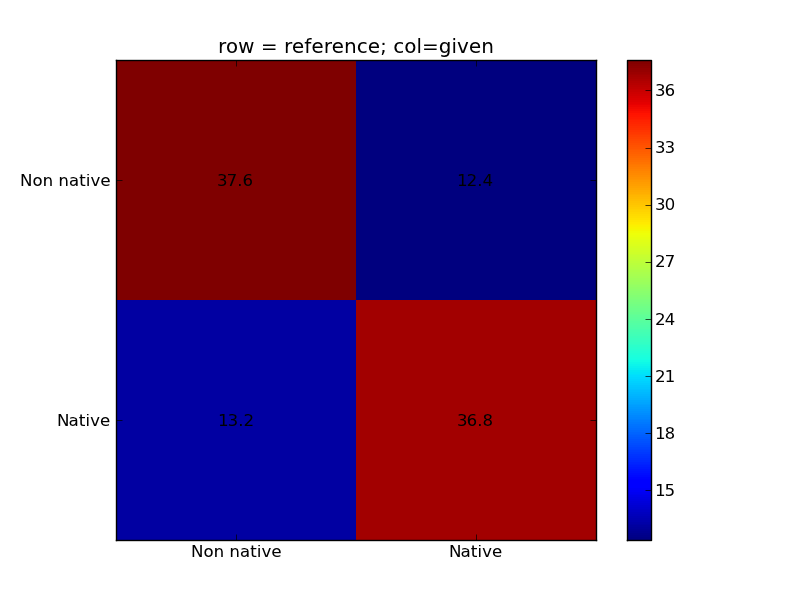
\includegraphics[scale=0.45]{native_cfm.png}
\caption{Native vs Non Native speakers experiment confusion matrix}
\label{non_cfm}
\end{figure}


The most informative features are words trigrams, words uni-gram, words bi-gram, words 4-gram, characters bigrams, PoS tags 4-grams, ordered by their importance. Table \ref{table:nonnative} shows the most correlated grams and speakers from the important features.

Some of the grams indicate possible common grammatical mistakes in the Non native speakers writing styles. Unigrams over words shows that non native speakers tend to use earth instead of Earth. Characters bigram shows that separating the comma from the previous word by a space is common usage of punctuation for non native speakers.
The usage of articles is a problematic issue for non native speakers, in the words 4-grams we can see using the article \emph{the} before a proper noun is a frequent pattern, this trend of using \emph{the} more than needed can be confirmed by the characters bigrams where \emph{th} appears. Word trigram shows that native speakers use \emph{the} correctly in \emph{in the middle} where we expect non native speakers to use \emph{in middle}.
Moreover, from the characters bigrams non native speakers use \emph{at} less than the native speakers which could suggest that they misuse the other articles where \emph{at} should be used. Characters bigrams shows a trend in spelling mistakes, where non native speakers type single \emph{l} instead of \emph{ll}. Another spelling trend is the less usage of apostrophes \emph{'}, this can be traced by the more frequent usage of \emph{am} in words unigrams for non native speakers and the appearance of \emph{don't} in the words 4-grams for native speakers.

\begin{table}[htp]
\begin{tabular}{l|ll}
	Feature & Speaker  & Gram
	\\\hline
	Words & Non Native &article on NNP\\
	 Trigrams& &  \verb+comma+ you have\\
	 & Native& used in the\\
	 &  &in the middle\\\hline
	 
	Words &Non Native& scene, To,\\
	   Unigrams&&describing, earth,\\
	    && referenced, am\\\hline
	    
	Words 	&Non Native& You have, we do\\
	Bigrams&& of people\\
	&Native& years of, I see\\
	&&if you\\\hline

	Words &Non Native& but I think that\\
	4-grams	&&by the NNP of\\
		&&( or at least\\
		&Native&NNP on NNP NNP\\
		&&if you don't\\\hline

	Characters&Non Native& th, e \verb+space+,\\
	Bigrams && \verb+space+ \verb+comma+\\
	&Native& l-, at, ll\\\hline
	
	PoS 4-gram &Non Native& NNS \textbf{,} DT NN\\
	&& MD VB VBN \textbf{,}\\
	&Native& \textbf{,} PRP VBZ JJ\\
	&& VBP NN IN NN\\
	
\end{tabular}
\label{table:nonnative}
\caption{Correlated grams and speakers for detecting non native speakers experiment}
\end{table}


\subsection{Frequent Languages Experiment}
This experiment aims to classify the speakers of the most frequent native languages. Six languages are selected US-EN, German, Spanish, French, Russian and Dutch. Figure \ref{pop_cfm} shows the confusion matrix of the logistic regression classifier. The data set size is about 150K comment. We can see clearly that the Russian users are the easiest to identify. Moreover, the classifier is the most confused distinguishing the German and the Dutch users with error $>2.0\%$ and to a less degree between (EN-US, French). These numbers confirm a basic intuition that the languages that have geographical proximity will have more borrowed words and grammars between them. This will affect their speakers writing styles in English.

\begin{figure}[htp]
\centering
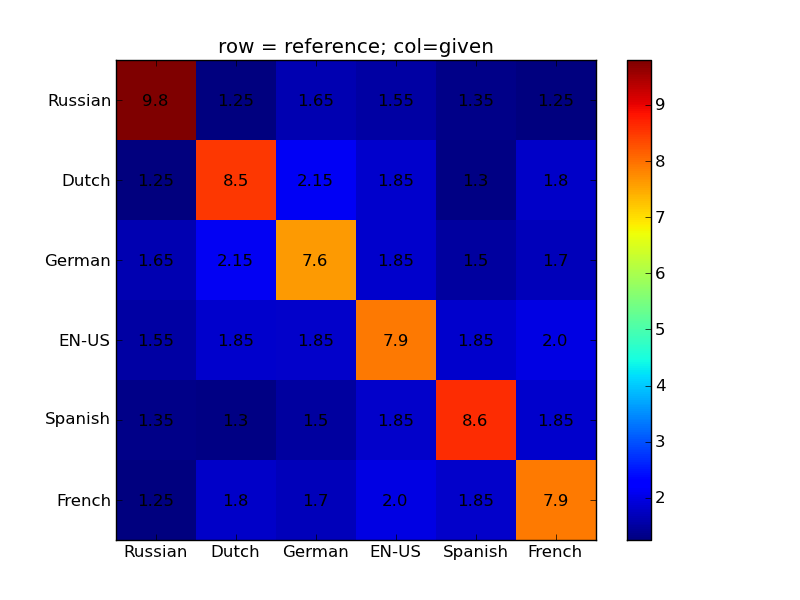
\includegraphics[scale=0.45]{popular_cfm.png}
\caption{Frequent languages experiment confusion matrix}
\label{pop_cfm}
\end{figure}

The most informative features are ordered as the following, words bigrams, words unigrams, words trigrams, characters 4 grams, words 4 grams, PoS tags 4-grams. We can see that the features of the longer grams become less informative once we increased the number of classes given to the classes. The increasing importance of shorter grams of words can indicate the influence of the topic of the comment on the classification.


\begin{table}[htp]
\begin{tabular}{l|ll}
	Feature & Speaker  & Gram
	\\\hline
	Words & Russian &prove that\\
	 Bigrams& German& you leave\\
	 & Spanish& to reveal\\
	 & Dutch & reliance on\\\hline
	 
	Words &Dutch& refuting\\
	   Unigrams&Spanish&timelines\\
	    &German& tie\\\hline
	    
	Words 	&Russian& stick to what\\
	Trigrams&Spanish& find out the\\
	&Dutch& end up in\\\hline

	Characters &French& hee \verb+space+\\
	4-grams	&French&ownr\\
		&Dutch&c/es\\
	\hline

	Words &French& NNP as far as\\
	4-grams &German& the NNP who\\
	&Spanish& ,etc),\\
	&EN-US& Does anyone know if\\\hline
	
	PoS 4-gram &Dutch& RB CD -RRB- IN \\
	&EN-US& VBD , RB DT\\
	&EN-US& CD VBD NNS IN\\
	
\end{tabular}
\label{table:nonnative}
\caption{Correlated grams and speakers for the most frequent languages experiment}
\end{table}


Table \ref{table:results} shows that the best accuracy that the classifier achieved is 50.27\% with 77K comment used. 
\subsection{Languages Families Experiment}

The confusion in classifying Dutch and German users suggests that there is a similarity between groups of languages. Referring to the linguistics research history of classifying the languages into families according to similar features and development history, this experiment tries to put such grouping under the microscope. 18 languages are grouped into 5 families as the following:
\begin{itemize}
\item Germanic\\
German, Dutch, Norwegian, Swedish, Danish.
\item Romanace\\
Spanish, French, Portuguese, Italian.
\item Uralic \\
Finnish, Hungarian.
\item Asian\\
Mandarin, Cantonese, Japanese, Korean.
\item Slavic
Russian, Polish
\end{itemize}

Figure \ref{fam_cfm} shows the that the Slavic and Asian native speakers has a clear style of writing English that is easy to detect relatively. The highest confusion in classification is between the Germanic and Romance languages, where geographical proximity plays a role in similarity. With the same reasoning we can see the confusion between Germanic and Uralic languages.

\begin{figure}[htp]
\centering
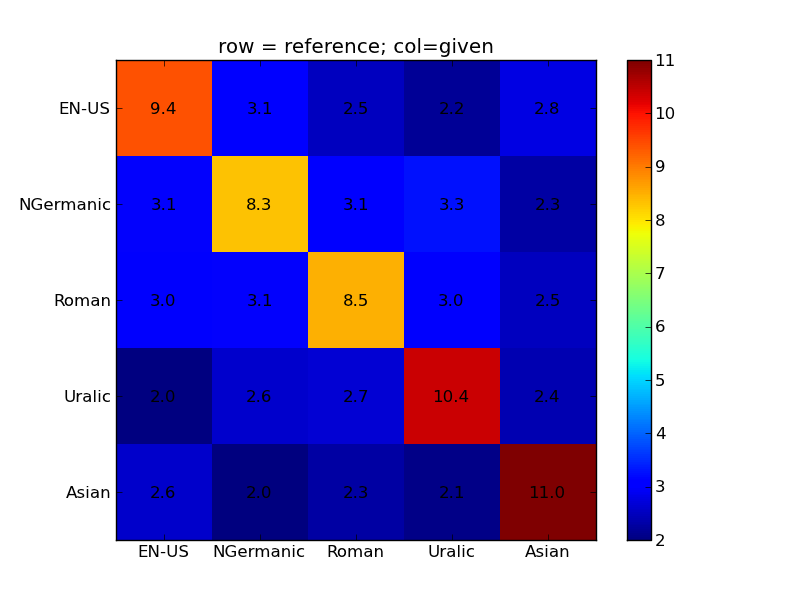
\includegraphics[scale=0.45]{family_cfm.png}
\caption{Languages families experiment confusion matrix}
\label{fam_cfm}
\end{figure}

Taking the opposite approach, we took the 20 languages and applied the same classification procedure over the new classes. The accuracy of the classifier is 25\%. However, considering the confusion matrix as a similarity matrix, we applied the affinity propagation clustering algorithm over the confusion matrix and the clusters that are formed are the following:
\begin{itemize}
\item Cluster 1: Arabic.
\item Cluster 2: Danish, Dutch, Finnish, Norwegian, Swedish.
\item Cluster 3: French, Italian, Portuguese, Spanish.
\item Cluster 4: Mandarin, Cantonese, Japanese, Korean.
\item Cluster 5: Russian, Polish, Turkish.
\item Cluster 6: Hungarian, German, US-EN.
\end{itemize}

The above clusters supports to large extent the literature classification of languages.

\subsection{Learning Algorithms}

Table \ref{table:results} shows negligible differences between different learning algorithms used in the experiments. 

\begin{table}[htp]
\begin{tabular}{l|ll}
	Experiment & Logistic Regression & Linear SVM
	\\\hline
	Non Native & 74.45\% & 74.53\%\\
	Frequent & 50.27\% & 50.26\%\\
	Families & 50.81\% &50.53\% \\
\end{tabular}
\caption{Accuracy of classification using different learning algorithms.}
\label{table:results}
\end{table}

Figure \ref{comb_lc} shows a typical over fitting situation where the more data you have the better the classifier can achieve. And here the size of data that can be extracted from Wikipedia plays a significant role to boosts the accuracy from 37\% to over 50\% in case of the Frequent languages and Families of languages experiments. The growth of the curve is similar to $\sqrt{x}$ curve which is similar to the growth of seen tokens in language models for English. This suggests the importance of the increase in the coverage of unique words to the performance of the classifier.

\begin{figure}[htp]
\centering
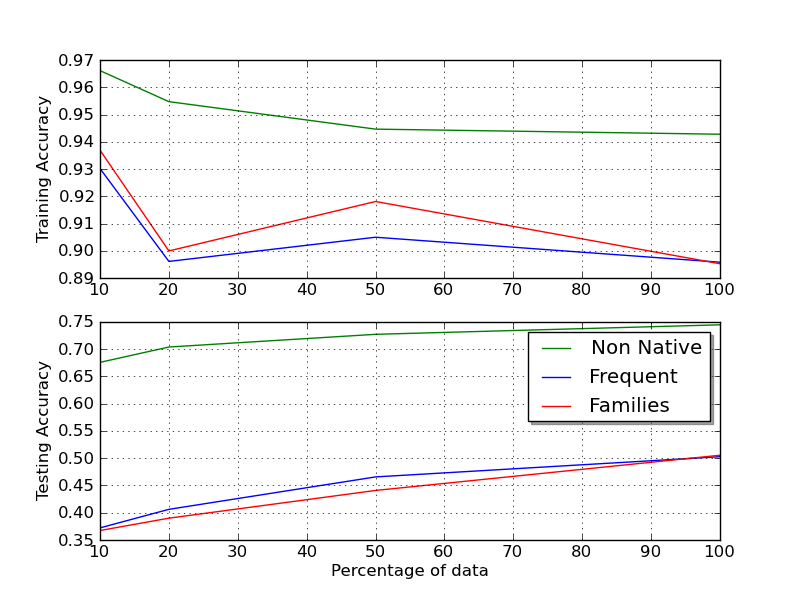
\includegraphics[scale=0.45]{combined_lc.png}
\caption{Learning curves of the logistic regression algorithm.}
\label{comb_lc}
\end{figure}





\section{Writing Styles}

Another type of Experiment focuses on the usage of PoS n-grams, trying to distinguish users by comparing the similarity of the PoS-ngrams distribution with a candidate language. We use the same definition of "similarity" as mentioned in the previous section and \cite {alpaydin2004introduction} and build a 20-classifier based on the whole training data (524 MB). After training our language model, The accuracy was around 95\% on training data.

The two baselines we selected are: Baseline-Max and Baseline-Random. Where in Baseline-Max we simply put each user into the category of native US English speaker since this class has the largest size with the
probability of about 34\%. And in Baseline-Random, we choose randomly from 20 candidate languages. The expectation of accuracy should be 5\%.

Since there exist some PoS-ngrams that might never appear in the training data, which means we have not seen such PoS-ngram before in any of the candidate category. We simply define these comments as "zero comments"--it is not precise to measure the value of these unseen PoS n-grams and we should put it into the category of native US English speaker to maximize the probability of correctness. Also, it sounds not reasonable if we consider comments that are too short considering the experiments mentioned in \cite {wagner2009judging}. So we first try on comments that has more than 100 PoS n-grams, which means the comment has more than (100+n-1) tokens.

\begin{table}[h]
\begin{center}
\small\addtolength{\tabcolsep}{-5pt}
\begin{tabular}{|l|l|l|l|l|}
\hline & \bf Overall & \bf Nonzero & \bf Available & \bf Nonzero \\ 
& \bf Accuracy & \bf Accuracy & \bf Count & \bf Count \\ \hline
4-grams & 35.47\% & 37.54\%  & 13067 & 8196 \\
tri-grams & 25.99\% & 25.96\% & 13209 & 13162 \\
bi-grams & 15.77\% & 15.77\%  & 13375 & 13375\\
uni-grams & 9.93\% & 9.93\%  & 13569 & 13569 \\
baseline-max & 34.03\% & 34.01\% & 13067 & 13067 \\
baseline-random & 5.00\% & 4.96\% & 13067 & 13067 \\
bag-of-words & 33.98\% & N/A & 13569 & 0 \\
\hline
\end{tabular}
\end{center}
\caption{\label{font-table} Result of Different PoS n-grams. }
\end{table}

It is clear from the table that the higher level of PoS n-grams, the higher the accuracy. But The experiment on 4-grams shows that about 1/3 of these comments contains unseen PoS 4-grams. Our training data contains more than 300,000 possible 4-grams in the category of native US English speaker, but that is still not enough, not to mention that the category of Korean native speaker only covers 18,000 4-grams. It seems that a good estimation of unseen PoS 4-grams can boost the accuracy. What's more, even word-unigram suffers the same problem (each comment with length greater than 100 had a token that was not seen anywhere before).

Another experiment runs on different length of comments using 4-grams, and we believe that the longer the comments, the higher the accuracy.

\begin{table}[h]
\begin{center}
\small\addtolength{\tabcolsep}{-5pt}
\begin{tabular}{|l|l|l|l|l|}
\hline Accuracy & \bf len$>$50 & \bf len$>$100 & \bf len$>$150 & \bf len$>$200 \\ \hline
4-grams & 33.18\% & 35.47\%  & 36.61\% & 37.57\% \\
baseline-max & 34.03\% & 34.01\% & 34.36\% & 35.04\% \\
baseline-random & 5.00\% & 4.96\%  & 5.01\% & 4.27\%\\
\hline
\end{tabular}
\end{center}
\caption{\label{font-table} Result of varies length overall. }
\end{table}

\begin{table}[h]
\begin{center}
\small\addtolength{\tabcolsep}{-5pt}
\begin{tabular}{|l|l|l|l|l|}
\hline Accuracy & \bf len$>$50 & \bf len$>$100 & \bf len$>$150 & \bf len$>$200 \\ \hline
4-grams & 33.40\% & 37.54\%  & 40.07\% & 42.24\% \\
baseline-max  & 34.75\% & 35.26\% & 36.15\% & 37.85\% \\
baseline-random  & 5.04\% & 4.67\% & 4.97\% & 4.22\% \\
\hline
\end{tabular}
\end{center}
\caption{\label{font-table} Result of varies length on nonzero data. }
\end{table}

We also observed that, some frequently appeared 4-grams occupy rather different portion in the distribution. For instance,
(IN,DT,NN,PRP): 0.13\% in Portugal but only 0.04\% in Korean
(NN,NN,IN,DT): 0.15\% in Portugal but only 0.05\% in Polish
(TO,DT,NN,IN): 0.11\% in Arabic while less than 0.06\% in any other languages
(',',CD,NNP,CD) and (NNP,CD,-LRB-,NNP): Appeared 10 times more in Korean than other languages, especially Hungarian.
(NN,PRP,VBZ,RB): Japanese and danish users prefer to use this.
 
Penalty for UNSEEN PoS-ngrams is too high and most of the time the correct answer was filtered at the first round, which means we never had a chance to calculate the similarity of distribution for the candidate. We also tried to apply different cutoffs in the experiment, which means we only count some frequent PoS-grams (without considering rare PoS n-grams) and avoid the possible spikes of weights in the process of learning. We tried to focus on most frequent k PoS 4-grams (k=100, 500, 2000, 5000) and those 4-grams appeared in more than k different candidate languages (k=10,15,20). As mentioned before, UNSEEN PoS-ngrams has some power in deciding some candidates languages, but the thresholds we found seems not as good as we expected.

\begin{table}[h]
\begin{center}
\small\addtolength{\tabcolsep}{-5pt}
\begin{tabular}{|l|l|}
\hline Accuracy & \bf 4-grams \\ \hline
no cutoff  &  37.54\% \\
most frequent 100 & 12.81\% \\
most frequent 500 & 15.26\% \\
most frequent 2000 & 21.76\% \\
most frequent 5000 & 30.55\% \\
appeared in 10 lang & 28.93\% \\
appeared in 15 lang & 32.27\% \\
appeared in all lang & 30.14\% \\
\hline
\end{tabular}
\end{center}
\caption{\label{font-table} Result of different cutoffs on PoS-ngrams }
\end{table}

To measure how ofter we throw away a correct answer, we eliminated all comments that contains unseen n-gram in the category of correct answer. After the tricky operation, we discarded about 3/4 of the available testing data, but we found a different result in the accuracy. In our tricky data, only 545 out of 2265 comments has unique candidate, and we got an accuracy of 78.41\% if the correct answer is not eliminated due to unseen PoS n-grams and probably compare between the candidate native language with US English. This phenomenon shows that the language model is reliable as long as we can calculate the distribution similarity. What's more, our model has a property of high precision and low recall. In our tricky data, the distribution of models output is:  

\begin{table}[h]
\begin{center}
\small\addtolength{\tabcolsep}{-5pt}
\begin{tabular}{|l|l|l|l|}
\hline & \bf Actual & \bf Predicted & \bf Correct \\ 
& \bf Occurrences & \bf Appearances & \bf Prediction \\ \hline
Deutsch & 181 & 150 & 78 \\
Japanese & 2 & 2 & 2 \\
Polish & 10 & 19 & 9 \\
Mandarin & 14 & 18 & 12 \\
Turkish & 4 & 4 & 4 \\
Finnish & 1 & 3 & 1 \\
Cantonese & 1 & 1 & 1 \\
Arabic & 14 & 13 & 13 \\
Danish & 11 & 18 & 10 \\
Hungarian & 4 & 4 & 4 \\
Spanish & 86 & 90 & 39 \\
Portuguese & 172 & 169 & 169 \\
French & 32 & 44 & 12 \\
Netherlands & 103 & 203 & 73 \\
US English & 1485 & 1329 & 1232 \\
Korean & 0 & 0 & 0 \\
Italian & 11 & 14 & 11\\
Swedish & 36 & 50 & 30 \\
Norwegian & 12 & 25 & 12 \\
Russian & 86 & 109 & 64 \\
\hline
\end{tabular}
\end{center}
\caption{\label{font-table} Statistics on tricky data }
\end{table}


while in the real data, we get hundreds of non-native speakers falling into the category of US English native speaker since this class covers more n-grams than the others.

In order to deal with unseen ngrams, we apply another method that can estimate the occurrance of a certain 4-gram by cascade down to using Trigram/Bigram/Unigram. But these attempts seems not Performing well, with only trigram/bigram estimation, the accuracy drop down to 34.5\%, and using only bigram/unigram estimation provide an accuracy of 29.7\%. If we apply both two strategies, the accuracy is 31.3\%. For most of the cases, cascade helps reduce the number of we predict some one as US English native, but it seldom solve the problem if the appearance of n-grams is really small, for instance, in Korean and Japanese. 

\section{Conclusions and Future Work}
As our results shows promising applications and trends using Wikipedia data to solve hard problems in robust means, there are many paths to improve our results and discover more interesting insights. We are looking to see the effect of increasing fluency of the non native speakers on their English language usage.

Moreover, as the learning curves show, it worth the effort increasing the size of the data in order of magnitude by adding the Wikipedia diffs, especially the non minor ones, as another source of users contributions. Moreover, the minimum size of the comments affects the performance of our classifiers, the relation between the quality of the data used and the accuracy of the classification is another interesting aspect.

The languages families experiments suggest the usefulness of using the English writing styles to define the similarities between different languages. This could lead to an interesting explanations and/or observations regarding the origins of some languages as Korean language which still a controversial topic.

Another direction is to solve the over fitting problem in our learning algorithms by applying smarter feature selection and adding more distinguishing features.

\section*{Acknowledgements}
We would like to thank Steven Skiena for the discussion and the advice. This work will not be available without the computing resources offered by his lab. We are also indebted to the NLTK and the Sklearn teams for producing excellent NLP and machine learning resources.

\bibliography{myrefs}{}
\bibliographystyle{acl}

\end{document}
